\section{Coordinate Frames}
In this investigation, Cartesian coordinate frames are employed to represent three-\\dimensional
vector quantities. These frames may remain fixed in space or rotate about their origin. Selection
of coordinate frame depends on the specific application as it can also be advantageous to either
position the origin at the center of mass of the system (barycenter) or align it with a primary
body of interest.

\subsection{The Barycentric Rotating Frame}
In a CR3BP system, the motion of a spacecraft is best illustrated within a rotating frame with the
origin at the system barycenter. The $\xhat$-axis is defined to extend from the barycenter toward
the smaller primary body, while the $\zhat$-axis aligns with the system angular momentum vector.
Completing the triad, the $\yhat$-axis is evaluated as $\yhat=\zhat\times\xhat$. This set of unit
vectors rotates about the barycenter at a constant angular rate $n$ identical to the mean motion of
the primaries. Consequently, the two primary bodies remain fixed in place in this frame.

\subsection{The Arbitrary Barycentric Inertial Frames}
The rotating frame is also defined relative to the arbitrary barycentric inertial (non-accelerating)
frame by an angle $\theta$. When $\theta=0$ (arbitrarily defined to be true when $t=0$ in the
time-autonomous CR3BP), the two frames are aligned and as time progresses, this angle increases as
the rotating frame revolves around the shared origin with $\thetadot=n$. The arbitrary inertial
frame is denoted with the right-handed unit vectors $\Xhat$, $\Yhat$, and $\Zhat$, where
$\Zhat=\zhat$. In \cref{fig:baryFrames}, the barycentric $\{\xhat,\yhat,\zhat\}$ rotating frame and
$\{\Xhat,\Yhat,\Zhat\}$ arbitrary inertial frame for a sample CR3BP system are illustrated, with
their common origin centered at the barycenter of the primaries, $P_{1}$ and $P_{2}$.

\begin{figure}[H]
    \centering
    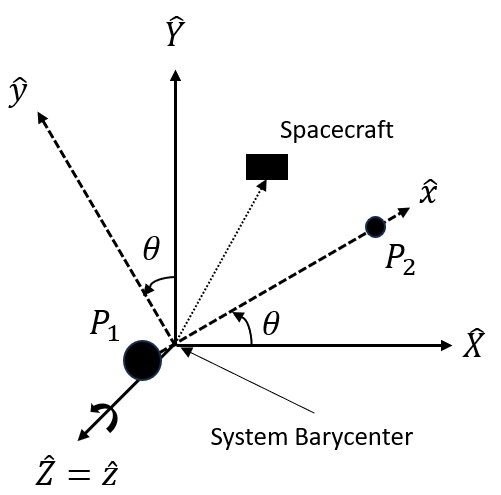
\includegraphics[width=0.5\textwidth]{figures/BaryFrames.jpg}
    \caption{Barycentric rotating and arbitrary inertial frames in a CR3BP system.}
    \label{fig:baryFrames}
\end{figure}

\subsection{The Ecliptic J2000 Primary-Centered Frame}
A commonly used primary-centered reference frame is the Ecliptic J2000. As the name implies, this
frame is defined with its origin at the center of Earth and the Sun-Earth orbital (ecliptic) plane
on January 1, 2000 as the $\Xhat_{Ec}\Yhat_{Ec}$-plane. The $\Xhat_{Ec}$-axis is directed towards
the vernal equinox, which is the line of intersection between the Earth's equatorial and ecliptic
planes on January 1, 2000. The $\Zhat_{Ec}$-axis is orthogonal to the ecliptic plane, and the
$\Yhat_{Ec}$-axis completes the triad, defined as $\Yhat_{Ec}=\Zhat_{Ec}\times\Xhat_{Ec}$. In this
investigation, the Ecliptic J2000 frame is utilized with its origin translated to the center of the
Sun, which is the shared primary body for the patched dynamical model. The construction of this
coordinate frame, as depicted in \cref{fig:eclipJ2000Frame}, is computed using the Navigation and
Ancillary Information Facility's (NAIF) SPICE ephemeris toolkit\cite{Semenov:2023}.

\begin{figure}[H]
    \centering
    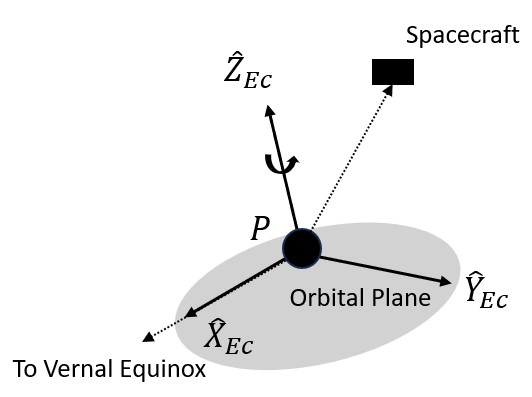
\includegraphics[width=0.5\textwidth]{figures/EclipJ2000Frame.jpg}
    \caption{Earth-centered Ecliptic J2000 frame.}
    \label{fig:eclipJ2000Frame}
\end{figure}
